\begin{tcolorbox}[
    colback=green!5!white, % Very light red background (5% red, 95% white)
    colframe=darkgreen!40!white, % Light red border (30% red, 70% white)
   title=Comparison of Ramsey and OLG, % Optional title
    fonttitle=\bfseries % Bold title
    ]

\begin{table}[H]
\centering
\renewcommand{\arraystretch}{1.4}
\setlength{\tabcolsep}{4pt}
\begin{tabularx}{\linewidth}{|>{\bfseries\RaggedRight\arraybackslash}p{2.8cm}|>{\RaggedRight\arraybackslash}X|>{\RaggedRight\arraybackslash}X|}
\hline
 & \textbf{Ramsey} & \textbf{OLG} \\
\hline
Demographics
  & Infinitely-lived households
  & Finitely-lived households \newline (two-period lifespan) \\
\hline
Heterogeneity
  & Homogeneous agents
  & Intergenerational heterogeneity \newline (young vs.\ old cohorts coexist) \\
\hline
Time
  & Continuous time \newline ($\rightarrow$ differential equations)
  & Discrete time \newline ($\rightarrow$ difference equations) \\
\hline
Welfare theorems
  & First Welfare Theorem holds: the competitive equilibrium coincides with the social planner's allocation
  & FWT may fail: dynamic inefficiency can arise, so the competitive equilibrium need not be Pareto optimal \\
\hline
Consumption smoothing
  & Intertemporal smoothing over an infinite horizon
  & Smoothing across the two phases of life via life-cycle savings \\
\hline
Period length
  & Calibration-dependent (typically one year)
  & Calibration-dependent (tied to the assumed length of a generation) \\
\hline
Foresight
  & Perfect foresight over an infinite horizon
  & Limited foresight: agents optimize only over their two-period lifespan \\
\hline
Representative agent
  & Admits a representative-agent formulation, either by symmetry or by aggregation across heterogeneous agents
  & No representative agent: aggregation fails due to overlapping cohorts \\
\hline
\end{tabularx}
\label{tab:ramsey-olg}
\end{table}
\textit{Note: If an representative agent exists a change in distribution between household does not change economic variables }
\end{tcolorbox}

    

\subsection{General Setup: Households and Firms}
\subsubsection{Households}
Individuals live for two periods: Youth $(i=y)$ during which one unit of labor is supplied (inelastically) and income is used for consumption now or savings for retirement $(i=o)$ during which the individual has to live off savings and interest payments. Life-time utility of an individual $(j)$ born at $t\in \mathbb{Z}$ is given by:
$$U_t = \frac{(C_{y,t})^{1-\sigma} - 1}{1-\sigma} + \frac{1}{1+\rho} \cdot \frac{(C_{o,t+1})^{1-\sigma} - 1}{1-\sigma}, \quad \sigma > 0, \ \rho \ge 0$$
The workforce is denoted by $L_t:=L_{y,t}$ and grows at rate $n\geq0$:
\begin{figure}[H]
    \centering
    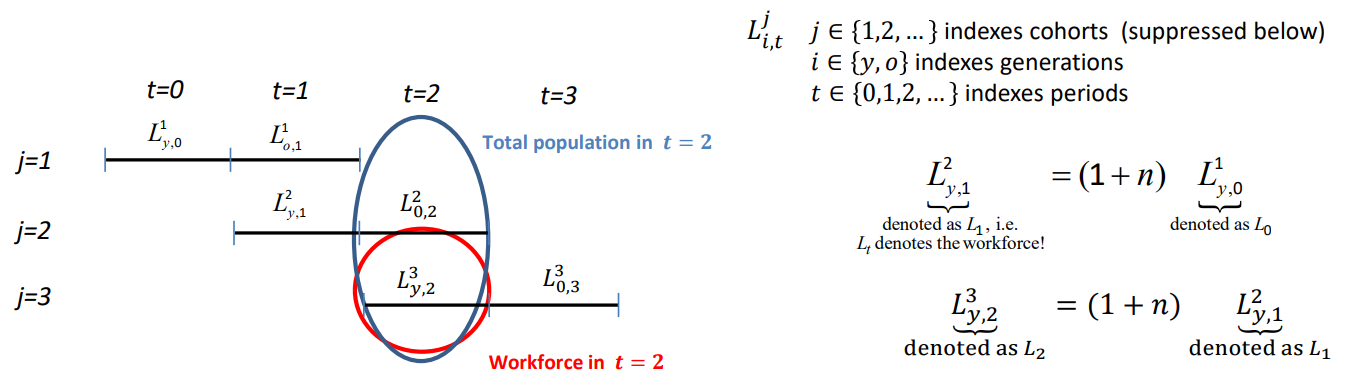
\includegraphics[width=0.7\linewidth]{olg.png}
    \label{fig:placeholder}
\end{figure}
\noindent \textit{Notice that an individual does not gain utility by inheriting wealth to its children.}
\subsubsection{Firms and Capital Accumulation}
Production is given by a constant returns to scale (CRS), i.e. $\lambda f(K,L)=f(\lambda K,\lambda L)$ technology with exogenous technological growth: 
$$Y_t=F(K_t,A_tL_t) \quad \quad A_t=(1+g)A_{t-1} \quad g\geq0$$
Setting $\lambda=1/(A_tL_t)$ we obtain the \textbf{intensive production function} $y_t=f(k_t)$, with $y_t:=Y_t/(A_t L_t)$ and $k_t:=K_t/(A_tL_t)$\\\\
Product and factor markets are \textbf{perfectly competitive}, i.e. firms make no profits in equilibrium and the \textbf{interest rate is: $r_t=f'(k_t)$}. Note that here, the depreciation rate is set to 0, i.e. $\delta=0$. \textbf{Real wage rate per $A_tL_t$ is: $w_t=f(k_t)-k_tf'(k_t)$}
\\\\
The capital stock is owned by the old and labor is supplied by the young. The \textbf{aggregate capital stock in period t is given by:} $K_t=S_{t-1}=\underbrace{L_{t-1}\bigl(w_{t-1}A_{t-1}-C_{y,t-1}\bigr)}_{\text{savings by the young generation at } t-1}$

\subsection{Household Dynamics}
\subsubsection{Households: Behaviour}
Maximization Problem of individual born at period $t$:
\begin{figure}[H]
\centering
\begin{minipage}{0.6\textwidth}
$$
\max_{\{C_{y,t},\, C_{o,t+1}\}} 
\frac{(C_{y,t})^{1-\sigma} - 1}{1-\sigma}
+ \frac{1}{1+\rho} \cdot \frac{(C_{o,t+1})^{1-\sigma} - 1}{1-\sigma}
$$

$$
\text{s.t. } \quad
C_{o,t+1} = (1 + r_{t+1}) \underbrace{\bigl(w_t A_t - C_{y,t}\bigr)}_{:=S_t}
\quad \Leftrightarrow \quad
0 = w_t A_t - \left( C_{y,t} + \frac{C_{o,t+1}}{1 + r_{t+1}} \right)
$$
\end{minipage}
\hfill
\begin{minipage}{0.35\textwidth}
\centering
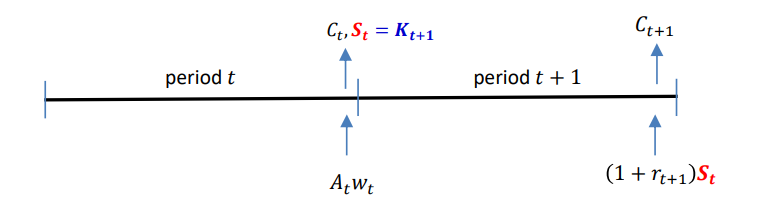
\includegraphics[width=\linewidth]{olghhtime.png}
\caption{Timing of events}
\end{minipage}
\end{figure}
\noindent Setting up the Lagrangian and solving for FOC: 
$$
\mathcal{L} :=
\frac{(C_{y,t})^{1-\sigma} - 1}{1-\sigma}
+ \frac{1}{1+\rho} \cdot \frac{(C_{o,t+1})^{1-\sigma} - 1}{1-\sigma}
+ \lambda_t \left[ w_t A_t - \left( C_{y,t} + \frac{C_{o,t+1}}{1 + r_{t+1}} \right) \right]
$$

$$FOC1: \quad
\frac{\partial \mathcal{L}}{\partial C_{y,t}}
= (C_{y,t})^{-\sigma} - \lambda_t = 0
\;\Rightarrow\;
(C_{y,t})^{-\sigma} = \lambda_t
$$

$$ FOC2: \quad
\frac{\partial \mathcal{L}}{\partial C_{o,t+1}}
= \frac{1}{1+\rho} (C_{o,t+1})^{-\sigma}
- \lambda_t \frac{1}{1 + r_{t+1}} = 0
\;\Rightarrow\;
(C_{o,t+1})^{-\sigma}
= \frac{1+\rho}{1 + r_{t+1}} \lambda_t
$$

$$ FOC3: \quad
\frac{\partial \mathcal{L}}{\partial \lambda}
= w_t A_t - \left( C_{y,t} + \frac{C_{o,t+1}}{1 + r_{t+1}} \right) 
$$

Dividing FOC2 by FOC1 yields the \textbf{Euler Equation} (analogue to two period discrete time Keynes-Ramsey rule): 
$$\frac{(C_{o,t+1})^{-\sigma}}{(C_{y,t})^{-\sigma}} = \frac{1+\rho}{1+r_{t+1}} \implies \frac{C_{o,t+1}}{C_{y,t}} = \left( \frac{1+r_{t+1}}{1+\rho} \right)^{1/\sigma}$$
\begin{itemize}
    \item Consumption increases whenever $r_{t+1}>\rho$
    \item Curvature of households utility function, i.e. intertemporal elasticity of substitution (given by $\sigma$) determines how much consumption varies in response to changes in $r_{t+1}-\rho$.   \textit{Note: This is also similar to the KRR in the Ramsey Model)}
    \item Log-linearization yields $\hat{C}\approxeq(r-\rho)/\sigma$
\end{itemize}
Together with the budget constraint, the Euler equation describes consumption with the \textbf{implied consumption function:}
$$C_{y,t} = [1 - s(r_{t+1})] w_t A_t \quad \text{with} \quad s(r_{t+1}) = \frac{(1+r_{t+1})^{(1-\sigma)/\sigma}}{(1+\rho)^{1/\sigma} + (1+r_{t+1})^{(1-\sigma)/\sigma}}$$



\begin{tcolorbox}[
    colback=red!5!white, 
    colframe=red!40!white, 
    title=Derivation of the savings rate and consumption, 
    fonttitle=\bfseries 
    ]
    \small
    \textbf{1. Euler Equation \& Budget Constraint} \\
    Multiple both sides of the Euler equation by $C_{y,t}$ and and get $C_{o,t+1} = \left( \frac{1+r_{t+1}}{1+\rho} \right)^{1/\sigma} C_{y,t}$ and substitute that into\\ $0 = w_t A_t - \left( C_{y,t} + \frac{C_{o,t+1}}{1+r_{t+1}} \right)$:
    \[
    0 = w_t A_t - C_{y,t} \left[ 1 + \frac{(1+r_{t+1})^{1/\sigma} (1+\rho)^{-1/\sigma}}{1+r_{t+1}} \right]
    \]

    \textbf{2. Solve for $C_{y,t}$} \\
    Using the identity $\frac{(1+r_{t+1})^{1/\sigma}}{1+r_{t+1}} = (1+r_{t+1})^{\frac{1-\sigma}{\sigma}}$:
    \[
    C_{y,t} \left[ \frac{(1+\rho)^{1/\sigma} + (1+r_{t+1})^{\frac{1-\sigma}{\sigma}}}{(1+\rho)^{1/\sigma}} \right] = w_t A_t
    \]
    \[
    C_{y,t} = \underbrace{\frac{(1+\rho)^{1/\sigma}}{(1+\rho)^{1/\sigma} + (1+r_{t+1})^{(1-\sigma)/\sigma}}}_{\text{consumption rate } 1-s} w_t A_t
    \]

    \textbf{3. Savings Rate Derivation} \\
    Since $s(r_{t+1}) = 1 - \frac{C_{y,t}}{w_t A_t}$:
    \[
    s(r_{t+1}) = 1 - \frac{(1+\rho)^{1/\sigma}}{(1+\rho)^{1/\sigma} + (1+r_{t+1})^{(1-\sigma)/\sigma}}
    \]
    \[
    s(r_{t+1}) = \frac{(1+\rho)^{1/\sigma} + (1+r_{t+1})^{(1-\sigma)/\sigma} - (1+\rho)^{1/\sigma}}{(1+\rho)^{1/\sigma} + (1+r_{t+1})^{(1-\sigma)/\sigma}}
    \]
    \[
    \mathbf{s(r_{t+1}) = \frac{(1+r_{t+1})^{(1-\sigma)/\sigma}}{(1+\rho)^{1/\sigma} + (1+r_{t+1})^{(1-\sigma)/\sigma}}}
    \]
\end{tcolorbox}

\subsubsection{Households: Savings Rate}
How does \textbf{interest rate} $r$ impact \textbf{savings rate} $s$?
\begin{figure}[H]
    \centering
    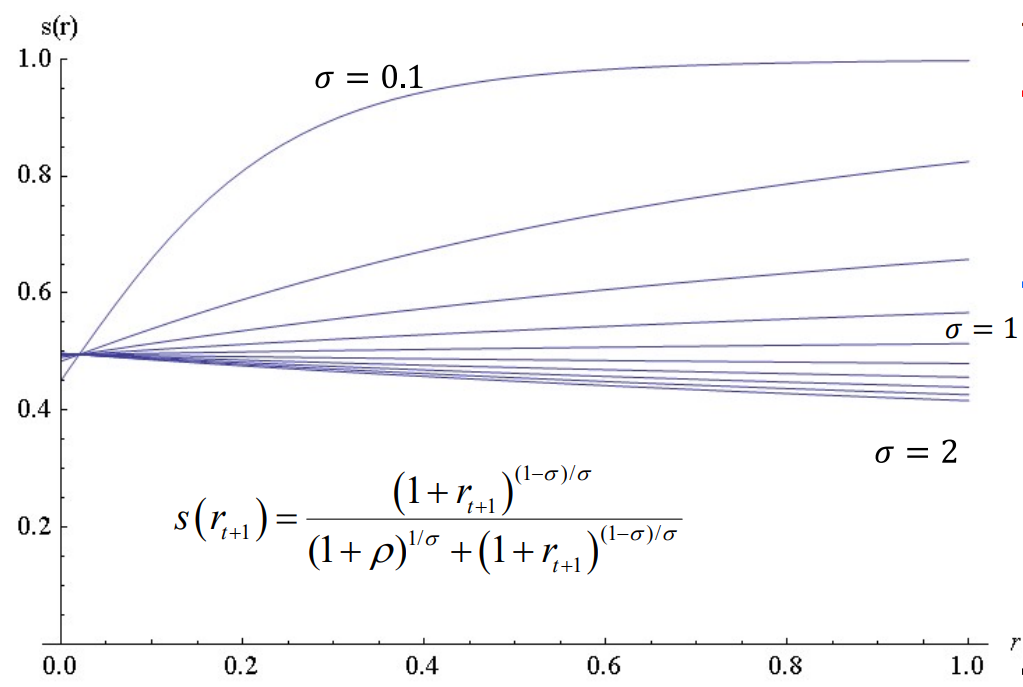
\includegraphics[width=0.6\linewidth]{savings.png}
    \label{fig:placeholder}
\end{figure}
\begin{itemize}
    \item \textbf{\textcolor{red}{Substitution effect.}} As $r$ increases, the opportunity costs of $C_1$ go up. Hence, $C_1$ is depressed and the \textbf{savings rate increases}: $r \uparrow \to C_1 \downarrow \to \textcolor{red}{s \uparrow}$
    
    \item \textbf{\textcolor{blue}{Income effect.}} As $r$ increases, capital income ($2^{nd}$ period of life) increases. Everything else the same, $C_2$ increases ($2^{nd}$ period income is completely consumed). Due to consumption smoothing, $C_1$ (out of labor income) goes up, meaning that \textbf{savings rate falls}: $r \uparrow \to (1+r)(wA - C_1) \uparrow \to C_2 \uparrow \to C_1 \uparrow \to \textcolor{blue}{s \downarrow}$
\end{itemize}
The \textbf{effect of $\sigma$} is, that ... .The savings rate $s(r_{t+1})$ is increasing in $r_{t+1}$ $\Leftrightarrow$ $ (1+r_{t+1})^{(1-\sigma)/\sigma}$ is increasing in $r_{t+1}$. \\
This is shown by: 
$$\frac{\partial (1+r_{t+1})^{(1-\sigma)/\sigma}}{\partial r_{t+1}} = \frac{1-\sigma}{\sigma} (1+r_{t+1})^{(1-\sigma)/\sigma - 1} = \frac{1-\sigma}{\sigma} (1+r_{t+1})^{(1-2\sigma)/\sigma}$$\\
We can look at three cases: 
\begin{itemize}[label={}]
    \item $$\frac{\partial s(r_{t+1})}{\partial r_{t+1}} > 0 \quad if \quad\sigma < 1$$
    \item $$\frac{\partial s(r_{t+1})}{\partial r_{t+1}} = 0 \quad if \quad \sigma = 1$$
    \item $$\frac{\partial s(r_{t+1})}{\partial r_{t+1}} < 0 \quad if \quad \sigma > 1$$
\end{itemize}

\subsection{General equilibrium and national accounting}
\textbf{Definition General Equilibrium:} A general (market) equilibrium for this economy consists of time paths for the \textcolor{blue}{quantities $\{K_t, Y_t, C_t\}_{t=0}^\infty$} and the \textcolor{red}{prices $\{w_t, r_t\}_{t=0}^\infty$} such that
        \begin{itemize}
            \item Final good producers maximize profits $Y_t - r_t K_t - w_t A_t L_t$ at each $t \in \{0, 1, \dots, \infty\}$
            \item Households maximize life-time utility
            \item    \text{Capital market clears: } K_t = S_{t-1} = L_{t-1}(w_{t-1}A_{t-1} - C_{t-1}) \,\, \forall \, t \in \{0, 1, \dots, \infty\} 
              \item  \text{Labor market clears: } L_t^S = L_t^D \,\, \forall \, t \in \{0, 1, \dots, \infty\} 
           \item Goods market clears: $Y_t + (1-\delta)K_t = I_t + C_t \ \forall \ t \in \{0, 1, \dots, \infty\}$ with $C_t = C_{y,t}L_t + C_{o,t}L_{t-1}$ (and $\delta = 0$ throughout this chapter)
        \end{itemize}
    \end{itemize}
\textbf{Goods market clearing condition}
$$
\underbrace{Y_t + (1-\delta)K_t}_{\text{goods available at end of } t}
= C_{o,t} + C_{y,t} + I_t
$$
$$
Y_t + (1-\underbrace{\delta}_{=0})K_t
= \underbrace{(1+r_t)\overbrace{s_{t-1} w_{t-1} A_{t-1} L_{t-1}}^{S_{t-1}}
}_{C_{o,t}}
+ \underbrace{(1-s_t) w_t A_t L_t}_{C_{y,t}}
+ \underbrace{s_t w_t A_t L_t}_{I_t = S_t = K_{t+1}}
$$
\\\\
\textbf{National accounting: $X_t = Y_t - \delta K_t$ // \textcolor{gray}{with $\delta = 0$}}
    \begin{itemize}
        \item National income $X_t$ (\textcolor{gray}{=total income of all households}) \textbf{equals} aggregate output $Y_t$.
        \item Noting $w_t = (1-\alpha)k_t^\alpha$, $r_t = \alpha k_t^{\alpha-1}$ and $k_t := K_t / (A_t L_t)$ gives
    \end{itemize}
\end{itemize}
\begin{align*}
X_t &= \underbrace{\underbrace{w_t}_{\text{wage per unit AL}} A_t L_t}_{\text{income of young agents}} + \underbrace{r_t K_t}_{\text{income of old agents}} = \underbrace{(1-\alpha) \left( \frac{K_t}{A_t L_t} \right)^\alpha}_{w} A_t L_t + \underbrace{\alpha \left( \frac{K_t}{A_t L_t} \right)^{\alpha-1}}_{r} K_t = K_t^\alpha (A_t L_t)^{1-\alpha}
\end{align*}

\subsection{Economy dynamics and capital accumulation}
Aggregate capital in $t+1$ is not-consumed output produced in $t$ and depends on $w_tA_t$ (wage income) and $r_{t+1}$ (expected interest rate). It is given by: 
$$ K_{t+1} = \underbrace{s(r_{t+1})w_t A_t}_{\text{savings per young agent}} \underbrace{L_t}_{\text{\# young agents}} \implies \underbrace{k_{t+1}}_{K_{t+1} / A_{t+1}L_{t+1}} = s(r_{t+1})w_t \frac{A_t L_t}{A_{t+1} L_{t+1}} $$
Since $A_{t+1}=(1+x)A_t$ and $L_{t+1}=(1+n)L_t$ we get: 
\begin{gather*}
k_{t+1} = \frac{1}{(1+x)(1+n)} s(r_{t+1}) w_t \\[2ex]
\text{Plug in competitive factor prices for $r_t$ and $w_t$}
\\
k_{t+1} = \frac{1}{(1+x)(1+n)} s \left[ \underbrace{f'(k_{t+1})}_{r_{t+1}} \right] \left[ \underbrace{f(k_t) - k_t f'(k_t)}_{w_t} \right]
\end{gather*}
This \textbf{first order difference equation}, together with the initial condition $k_0=k_{initial}$ describes the evolution of the economy. We can find the \textbf{zero growth steady state} in $\tilde{k}=K/(AL)$, where $\tilde{k}=k_t=k_{t+1}$
$$\tilde{k} = \frac{1}{(1+x)(1+n)} s \left[ f'(\tilde{k}) \right] \left[ f(\tilde{k}) - \tilde{k} f'(\tilde{k}) \right]$$
\begin{itemize}
    \item $k_t=const.$ implies $\frac{K_{t+1}}{K_t}=(1+x)(1+n)$
    \item In steady state we have $s=const.$ and $K/Y=const.$
\end{itemize}\\

Plugging $y=k^\alpha$ and $\sigma=1$ into our difference equation above, yields: 
$$k_{t+1} = \frac{1}{(1+x)(1+n)} \frac{1}{2+\rho} (1-\alpha) k_t^\alpha$$
\begin{minipage}{\textwidth}
    % Linke Seite: Das Bild
    \begin{minipage}{0.45\textwidth}
        \centering
        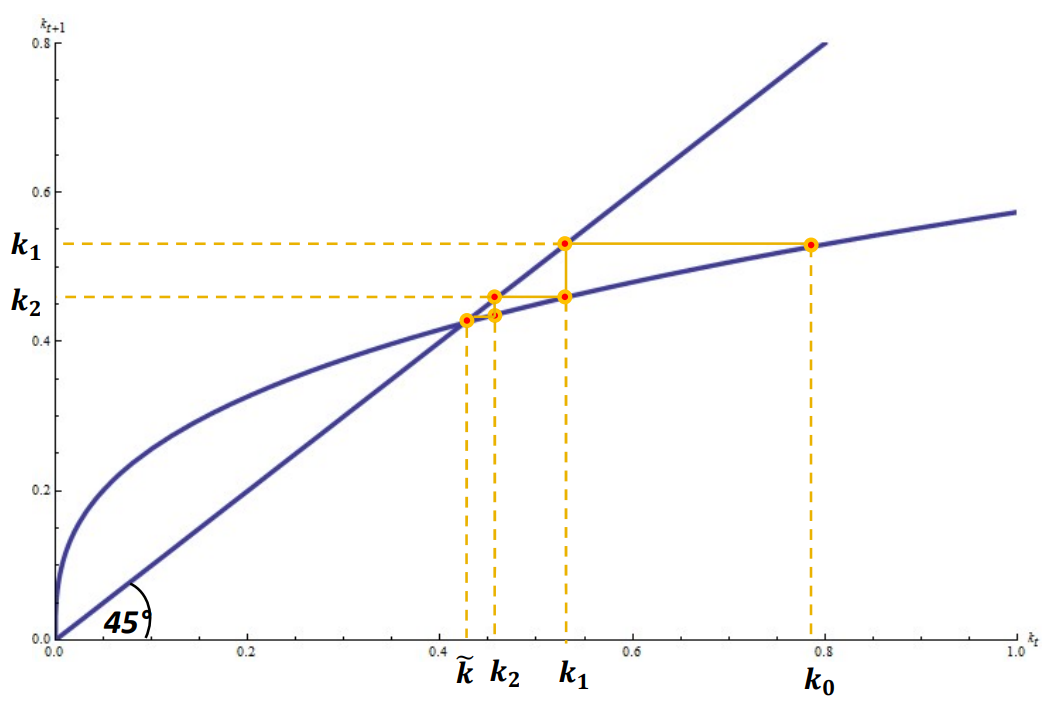
\includegraphics[width=\linewidth]{olgdyn.png}
        \label{fig:olgdyn}
    \end{minipage}
    \hfill % Erzeugt Abstand zwischen den Minipages
    % Rechte Seite: Der Text
    \begin{minipage}{0.5\textwidth}
        \begin{itemize}[leftmargin=*]
            \textbf{Special case with \textit{logarithmic utility} and \textit{Cobb-Douglas} technology}
            \begin{itemize}
                \item For $\sigma = 1$, we get $s = \frac{1}{(2+\rho)}$. Moreover, under Cobb-Douglas $f(k) = k^\alpha$ and $w = (1-\alpha)k^\alpha$.
                \item Any parameter change that raises savings rate (e.g. negative shock to $\rho$) shifts balanced growth path upward but leaves long-run growth rate unaffected.
            \end{itemize}
        \end{itemize}
    \end{minipage}
\end{minipage}


\subsubsection{Dynamic Inefficiency}

In the steady state, the condition $\tilde{r} = n + x$ represents a boundary ('growth speed limit') where consumption is maximized ($\rightarrow$ Golden Rule). Unlike the Ramsey model, the OLG framework allows for \textbf{dynamic inefficiency}, where an economy over-accumulates capital such that $\tilde{r} < n + x$. In this scenario, reducing the savings rate actually increases consumption $\tilde{c}$ for all generations.
\\
Consider the  OLG model with a Cobb-Douglas production function $y = k^\alpha$, and the simplifications $x=0$, $\delta = 0$, and $\sigma=1$ (log-utility). The steady-state capital per effective worker $\tilde{k}$ is:
\begin{equation*}
\tilde{k} = \left( \frac{1}{1+n} \frac{1}{2+\rho} (1-\alpha) \right)^{\frac{1}{1-\alpha}}
\end{equation*}
\noinent Plugging this into the marginal product of capital $f'(\tilde{k}) = \alpha \tilde{k}^{\alpha-1}$ yields the equilibrium interest rate:
\begin{align*}
\tilde{r} &= \alpha \left[ \left( \frac{1}{1+n} \frac{1}{2+\rho} (1-\alpha) \right)^{\frac{1}{1-\alpha}} \right]^{\alpha-1} \\
&= \frac{\alpha}{1-\alpha} (1+n)(2+\rho)
\end{align*}
\noindent Note that $r=f'(k)$ and $x=0$. \\
We evaluate efficiency by comparing this market rate to the Golden Rule level $r_{GR}=f'(\tilde{k}_{GR}) = n+0$
\begin{itemize}
    \item \textbf{Efficient Region:} $\tilde{r} \geq n$. The market accumulates an optimal or sub-optimal amount of capital.
    \item \textbf{Inefficient Region:} $\tilde{r} < n$. This occurs if $\alpha$ is sufficiently small. In this case, $\tilde{k} > \tilde{k}_{GR}$, meaning the economy is "saturated" with capital.
\end{itemize}
\noindent The First Fundamental Theorem of Welfare (FTW) fails here because the infinite horizon of the economy, combined with the finite lives of agents, allows the competitive market solution to persist in a state of Pareto-inferior over-accumulation.
\\\\
\textbf{Intuition behind dynamic inefficicency}
\begin{itemize}    
        \item \textbf{Overaccumulation:} It arises when a society saves "too much," leading to a capital stock so large that the marginal product of capital falls below the economy's growth rate ($r < n$).
        \item \textbf{Pareto improvement:} In this state, the economy is wasteful. A transfer scheme (reducing current savings to pay for current elderly consumption) can make every generation better off without reducing future consumption.
        \item \textbf{Pecuniary Externalities:} Individual households save for their own old age without considering that aggregate overaccumulation drives down the interest rate for everyone. 
        \item \textbf{Market Failure:} Because the economy involves an infinite horizon with infinite agents, the First Welfare Theorem does not hold, allowing for competitive equilibria that are not Pareto optimal.
    \end{itemize}
\end{itemize}


\begin{tcolorbox}[
    colback=blue!1!white,
    colframe=blue!40!white,
    title=Dynamic Inefficiency: From Solow to Ramsey to OLG,
    fonttitle=\bfseries
    ]
The dynamic inefficiency condition $\tilde r < n + x$ is \textbf{not new}, but the same Golden Rule condition we know from the Solow model. What is new in OLG is that the market equilibrium can fall into the inefficient region all by itself.
\\\\
\textbf{Solow recap.:} Raising the savings rate rotates the savings curve $sf(\tilde k)$ upward, shifting the intersection with the break-even investment line $(n+x+\delta)\tilde k$ to the right. This results in a higher steady-state capital intensity $\tilde k^*$. However, any capital stock to the right of the Golden Rule level $\tilde k_{\text{gold}}$ is considered dynamically inefficient: due to diminishing returns, $f'(\tilde k)$ falls and so does the interest rate. The economy over-accumulates until the net rate falls below the growth rate, i.e., $\tilde r < n + x$. The Golden Rule itself reads
\[
    \underbrace{\tilde r + \delta}_{f'(\tilde k)} = \delta + n + x \iff \tilde r = \underbrace{n+x}_{\hat Y = g}.
\]

\begin{figure}[H]
    \centering
    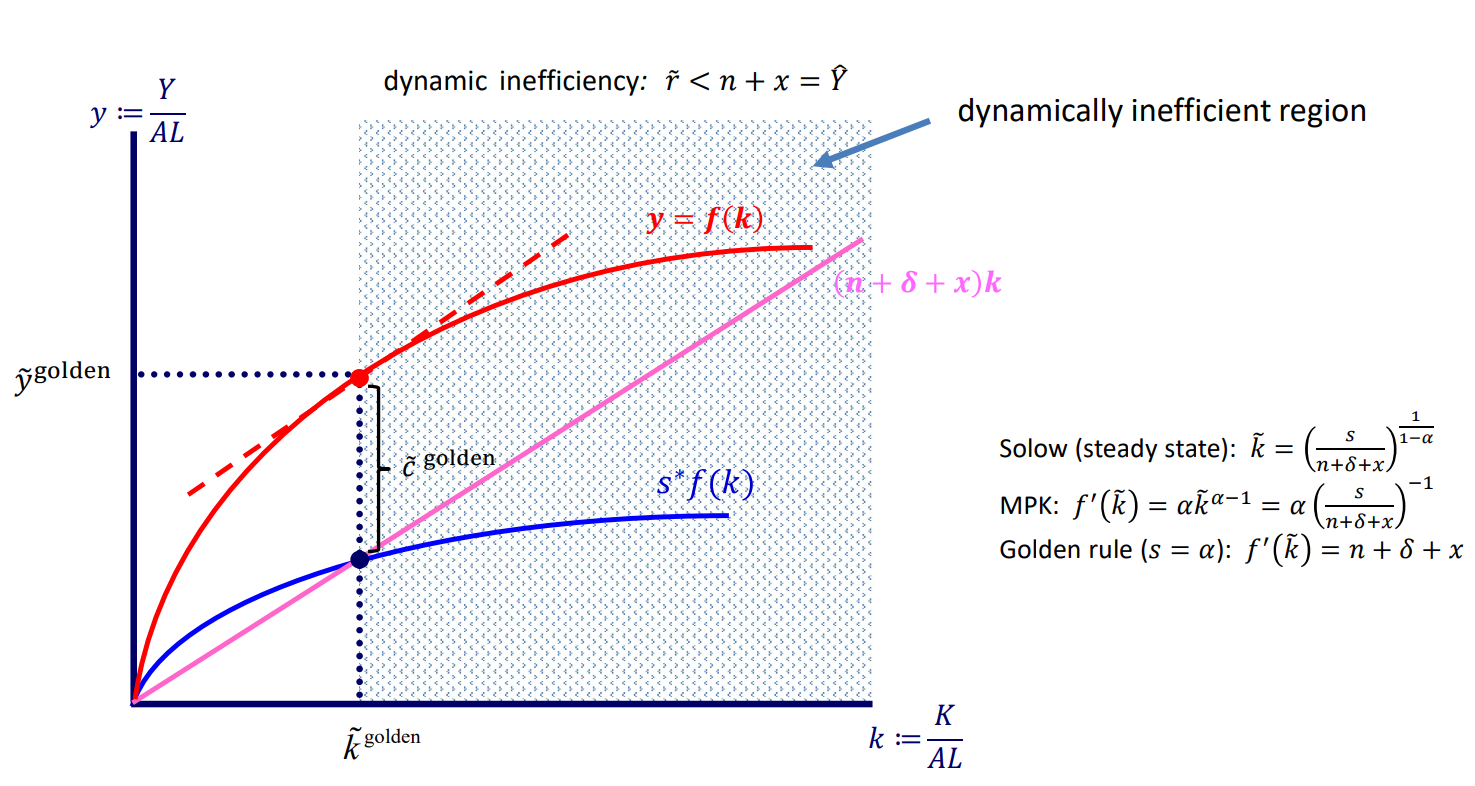
\includegraphics[width=0.8\linewidth]{solowolg.png}
    \label{fig:placeholder}
\end{figure}

\textit{Comparing the three models.} The same Golden Rule benchmark $\tilde r = n+x$ plays a different role in each framework:
\begin{itemize}
    \item \textbf{Solow.} The savings rate $s$ is exogenous. If you choose $s$ above $s_{\text{gold}} = \alpha$, the steady state lies to the right of $\tilde k_{\text{gold}}$ and $\tilde r < n+x$. Inefficiency is the \textbf{modeller's choice}: pick a different $s$ and the problem disappears.
    \item \textbf{Ramsey.} The savings rate is endogenous and chosen by an optimizing household. The TVC rules out paths with $\tilde r < n+x$ (these violate dynamic optimality, as discussed in the saddle-path analysis). The First Welfare Theorem holds, and the equilibrium is always on the efficient side: $\tilde r \geq n+x$ 
    \item \textbf{OLG.} The savings rate is also endogenous, but the optimization is only over a \textit{two-period} life. The young save for retirement without internalizing that aggregate over-saving drives down the future interest rate (a \textbf{pecuniary externality}). The First Welfare Theorem fails, and $\tilde r < n+x$ can persist as a competitive equilibrium. Compare the OLG market rate
    \[
        \tilde r = \frac{\alpha}{1-\alpha}(1+n)(2+\rho)
    \]
    to the golden rule: $n+x$. If the market rate is lower, the economy is dynamically inefficient. 
\end{itemize}

\textbf{Why does Ramsey not have the same problem like OLG?} The infinitely-lived Ramsey household weighs the marginal cost of saving today against \textit{all} future consumption benefits. If $r < \rho$, the household simply stops saving. In OLG, the young household only weighs saving against \textit{its own} retirement consumption -- the indirect effect on future generations through capital accumulation is invisible to the saver. This generational disconnect is the source of the market failure.
\end{tcolorbox}



\begin{tcolorbox}[
    colback=blue!1!white,
    colframe=blue!40!white,
    title=Derivation of the optimal savings rate in the Solow model,
    fonttitle=\bfseries
    ]
The Golden Rule savings rate $s_{\text{gold}}$ is the savings rate that maximizes steady-state consumption per effective worker $\tilde c$.

\textit{Setup.} Consider the Solow model with Cobb-Douglas production $y = k^\alpha$, exogenous labor growth $n$, technological progress $x$, and depreciation $\delta$. The steady-state capital intensity is
\[
    \tilde k = \left(\frac{s}{n+\delta+x}\right)^{\frac{1}{1-\alpha}},
\]
and steady-state consumption per effective worker is
\[
    \tilde c(s) = (1-s)\, \tilde k(s)^\alpha = \tilde k(s)^\alpha - (n+\delta+x)\, \tilde k(s),
\]
where the second equality uses the steady-state condition $s\, \tilde k^\alpha = (n+\delta+x)\,\tilde k$.

\textit{Maximization.} Differentiate $\tilde c$ with respect to $\tilde k$ and set equal to zero:
\[
    \frac{d\tilde c}{d\tilde k} = \alpha \tilde k^{\alpha-1} - (n+\delta+x) = 0 \quad \Longrightarrow \quad \underbrace{\alpha \tilde k^{\alpha-1}}_{f'(\tilde k)\, =\, \tilde r + \delta} = n+\delta+x.
\]
Rearranging gives the \textbf{Golden Rule condition}:
\[
    \boxed{\; \tilde r = n + x \;}
\]
i.e., the net marginal product of capital equals the economy's growth rate $\hat Y = n + x$.

\textit{Solving for $s_{\text{gold}}$.} Plug the steady-state expression for $\tilde k$ into the Golden Rule condition $\alpha \tilde k^{\alpha-1} = n+\delta+x$:
\[
    \alpha \left(\frac{s}{n+\delta+x}\right)^{-1} = n+\delta+x \quad \Longrightarrow \quad \alpha \cdot \frac{n+\delta+x}{s} = n+\delta+x.
\]
Solving for $s$:
\[
    \boxed{\; s_{\text{gold}} = \alpha \;}
\]
i.e., the Golden Rule savings rate equals the capital share. Empirically $\alpha \approx 0.3$.

\textit{Interpretation.}
\begin{itemize}
    \item If $s < \alpha$: the economy under-saves; raising $s$ raises steady-state $\tilde c$.
    \item If $s = \alpha$: steady-state consumption is maximized.
    \item If $s > \alpha$: the economy over-saves and is in the \textbf{dynamically inefficient region}; lowering $s$ raises $\tilde c$ for all generations (a Pareto improvement).
\end{itemize}
The Solow model treats $s$ as exogenous, so reaching $s_{\text{gold}}$ is a matter of policy / modeller's choice. In Ramsey, the household's optimization rules out $s > \alpha$ via the TVC; in OLG, however, $s > \alpha$ can arise as a competitive equilibrium outcome.
\end{tcolorbox}
